\documentclass          {article} % For LaTeX2e
\usepackage             {amsmath}
\usepackage             [center]
                        {caption}
\usepackage               {subcaption}
\usepackage             {nips15submit_e,times}
\usepackage             {graphicx}
\usepackage             {hyperref}
\usepackage             {url}
%\documentstyle[nips14submit_09,times,art10]{article} % For LaTeX 2.09

\title                  {Higgs Machine Learning Challenge \\with Neural Network Adversarial Training}

%\author{
%
%\And
%
%\AND
%
%}

%\textbf{Oren Shklarsky}\\
%Department of Physics\\
%Simon Fraser University\\
%Burnaby, BC V5A 1S6\\
%\texttt{oshklarsky@sfu.ca}\\

%\textbf{Darren Temple}\\
%Department of Physics\\
%Simon Fraser University\\
%Burnaby, BC V5A 1S6\\
%\texttt{dtemple@sfu.ca}\\

%\textbf{Morgan Jenkins}\\
%Department of Computer Science\\
%Simon Fraser University\\
%Burnaby, BC V5A 1S6\\
%\texttt{mjenkins@sfu.ca}\\

\newcommand             {\fix}{\marginpar{FIX}}
\newcommand             {\new}{\marginpar{NEW}}

%\nipsfinalcopy % Uncomment for camera-ready version

\begin                  {document}

\maketitle

% **************************************************************************************************************************

\begin                  {abstract}
The Higgs particle was theorized in 1964 and finally discovered in 2012 by the ATLAS and CMS experiments at CERN. This particle is the keystone of the Standard Model of particle physics, and provides the mechanism by which other particles acquire mass. Such discoveries are statistical in nature, and require vast amounts of information from the debris of particle collisions. Sifting and categorizing this data is a continual challenge, and in 2014 CERN and Kaggle invited the public to try their hand at such work in the "Higgs Machine Learning Challenge". A number of top entries used neural networks, including the winner. An extended approach using the so-called "adversarial training" technique is presented herein.
\end                    {abstract}

% **************************************************************************************************************************

               \section {Introduction}
               \label   {sec:introduction}

%%Particle physics arguably began with the discovery of the electron by J.J. Thomson in 18?? \cite{???}. This began a century of subsequent rapid discoveries of new particles, next being the identification of the proton in 19?? \cite{???} and then the neutron in 19?? \cite{???}, both by Ernest Rutherford. These three particles - electron, proton and neutron - are all that's needed to build the everyday chemical elements that comprise the apparent material universe. However, it was with early studies of cosmic rays that our understanding of fundamental particles began to change. One after the other more and more particles were discovered, with a broad spectrum of characteristics. Patterns slowly emerged, leading to the so-called Standard Model of particle physics, which encompasses not only particles of a material nature but also particles that transmit the very forces between them, thereby enabling their interactions.

Alongside the well-known types of material and force-carrying particles, the Standard Model of particle physics has an altogether different type of entity, which was theorized to exist in order to explain why certain particles have mass. This came to be known as the Higgs particle, named after the author of the groundbreaking 1964 paper by one of the pioneers of this field \cite{???}. So began a search that spanned nearly four decades, culminating with the discovery of the Higgs particle in 2012 by the ATLAS and CMS experiments, which operate at the Large Hadron Collider (LHC) at the CERN lab in Geneva \cite{???}. The tell-tale signals were given by the physics properties of the Higgs particle's decay products, as the particle itself cannot be directly observed due to decaying so rapidly that it cannot travel out of its creation region and into the detector.

%%There are two main abilities of the experimental apparatus that allowed for the Higgs particle to be discovered, that were not had with earlier experiments.
%%Energy is the raw ingredient of all particles, in other words, and different particles require different amounts of this ingredient.
First and foremost for this discovery to happen was the particle collision energy, and second was the ability of the detectors to record and analyze data. Every particle has a characteristic mass energy, and this energy must be met by a device such as the LHC in order for the particle to be created. The Higgs particle happens to be a relatively massive particle compared to a number of others, and therefore requires a relatively large amount of energy. A technological evolution over many years and many generations of device was necessary to develop the LHC, which is powerful enough to provide the Higgs creation energy.

%%Originally, detectors were comprised of some continuous medium that would reveal a particle track that could be photographed and measured by hand.
%%Things have come a long way since early detectors, with modern devices being formed of multiple layers of electronics, each sampling the outgoing decay products in different ways.
Once created, a high mass particle such as the Higgs rapidly decays into other, lighter particles, which may themselves decay further. A variety of these decay products that are detected and categorized by such properties as momentum and electric charge, based on their trajectories through the machine. This data is then used to infer the ancestral particle at the initial creation point.

%%as used to be possible in photographic detectors from previous generations
Despite the LHC providing an appropriate energy range for the creation of Higgs particles, their production is still exceedingly rare compared with the production of a number of other particles. An exceedingly large number of creation events is therefore required to compensate for the rarity, and the particle tracks simply cannot be assessed individually. The vast stream of electronic readout must be dealt with computationally and statistically, and a great deal of time and effort is spent by scientists determining how best to seek the signals of interest.

%%, following the reconstruction of particle properties from the raw signal,
Machine learning has inevitably become invaluable for this task, which is simply one of classification, namely a question of signal versus background. In the case of the Higgs particle, its various decay channels are not unique, and are in fact shared by the decays of other heavy particles. Seeing a certain set of decay products does not then give indisputable proof of one particular ancestor particle or the other. But there are nonetheless subtle signs within the data when viewed \textit{en masse}, which machine learning algorithms can be trained to recognize.

%Tau particles are heavier versions of electrons, and just like other heavy particles they also decay into a range of products that enter the detector. It is therefore these decay products that are used to infer the taus, and the taus are then used to infer Higgs particles.

%%Many technical fields are developing incredibly fast at present, and machine learning is no exception. Even just more than one year on from the Higgs machine learning challenge, new ideas and techniques have become available. This project seeks to explore one such technique that has started to generate a lot of interest of late, namely that of adversarial training, and to apply it to the HMLC.

% **************************************************************************************************************************

               \section {Higgs Machine Learning Challenge}
               \label   {sec:higgs_machine_learning_challenge}

In 2014, CERN scientists collaborated with the Kaggle machine learning organization, developing an open competition for the public to try and develop a machine learning classifier to distinguish the Higgs particle from other heavy particles in the tau-tau decay channel \cite{???}. This was the Higgs Machine Learning Challenge (HMLC), which at the time of its release was the most popular Kaggle challenge up to that point, with a total of 35,772 uploaded entries submitted by 1,785 teams (1,942 people) comprised of participants from around the world, some working within the physics community, others simply interested in computing \cite{Rousseau2015}. The winning entry came from a sole programmer with no advanced physics training, who developed a neural network model that was clearly superior to anything else \cite{Rousseau2015}.

%%Despite machine learning being a key component to many physics analyses at CERN, there is relatively little development of these techniques within the organisation itself \cite{Rousseau2015}. When one technique is found to work and is well understood, and, crucially, it is well understood how to interpret the resulting physics results, then that technique gets entrenched and remains in play for a long time. This is not a bad thing in many ways, as by having staple workhorse codes it is possible for physicists to spend a greater fraction of their time analysing the data in search of physics.

%%However, machine learning is a field in its own right, and has its own experts and development trends quite separate from any of its applications, in science or otherwise. The last decade in particular has seen an enormous rise in both the ability of machine learning and the applications \cite{Rousseau2015}. An ever increasing fraction of the developed world's activities has some computational aspect, and with that comes more data and more need to analyse that data for patterns. Coupled with this is the increase in the ability of hardware to run ever more complicated algorithms, making theoretical work from previous generations of computer science suddenly more relevant and useful.

%%The Higgs Machine Learning Challenge (HMLC) was develped in order to tap into the knowledge of this field straight from the enthusiasts, in order to port that knowledge into the particle physics domain. This is not only beneficial for CERN, but also the machine learning community at large, which demands as many real world problems as possible in order to develop the most relevant algorithms \cite{Rousseau2015}. Sourcing good data is a job in itself, and if there's one thing that CERN is good at it's generating data. The HMLC was therefore a mutually beneficial arrangement for the data generation experts and the data processing experts.

The HMLC has two datasets - one fully labelled dataset for training, and another unlabelled dataset for testing. The training dataset has information about 250,000 labelled events, and the testing dataset corresponds to 550,000 unlabelled events. The labels are simply "signal" and "background". In a particle physics collider, two input particles (protons in the case of the LHC for ATLAS and CMS experiments) are accelerated and collided at high speed, resulting in a high energy state that can form any particle which "costs" that amount of energy or less. Call this created particle the \textit{initial state}. This initial state often has a number of possible decay channels to some set of \textit{final state} particles, and some initial states share similar final states. In the case of the Higgs particle, one decay channel is that to a pair of lighter tau particles, with these then decaying to yet lighter particles still. These events are those labelled as "signal". Such final states are possible from the decay of other initial states such as W and Z particles (which are the carriers of the weak force) and top particles (which are the heaviest of the quark family) \cite{Rousseau2015}. These events are those labelled as "background".

%% (which are particles within the family of the constituents of protons and neutrons)
%%, which are not directly detected but inferred via a deficit in the energy accounting
It is the subtle differences in the ensemble physics variables that we seek to distinguish through machine learning. Both training and testing datasets are defined by a feature set comprised of 30 different physics variables, representing quantities such as the mass, energy and momentum of decay products that entered the detector or were otherwise inferred \cite{Rousseau2015, Chen2015}. These entities are either (1) electrons, (2) heavier variants of electrons (muons and taus), (3) jets of particles comprised of quarks, and (4) so-called missing energy, representing very light and weakly interacting particles called neutrinos \cite{Chen2015}.

%%who have to carefully reconstruct such high level output from a very low level input.
%%Furthermore, the dataset is in fact the product of a very fine Monte Carlo simulation, of the sort that is actually used for understanding the background in real data.
Physics details aside, this format of problem is ubiquitous in machine learning, and requires no knowledge or understanding of what the features actually are. The HMLC dataset is actually a vastly simplified version of Monte Carlo simulated data used by CERN physicists. It was carefully tailored to be simply enough for public use, but still interesting enough to promote useful machine learning techniques \cite{Rousseau2015}. The signal to background ratio in the HMLC dataset is much larger than that in real data, which requires many millions of events in order to provide statistically significant findings, so being impractical for the HMLC.

% **************************************************************************************************************************

               \section {HMLC Winner and Initial Impulse}
               \label   {sec:hmlc_winner_and_initial_impulse}

As mentioned in \S\ref{sec:introduction}, there were many hundreds of entrants to the original Kaggle competition, with the overall winner being a single programmer with no professional physics training, specializing instead in computational development and consulting \cite{Rousseau2015}. In fact, the physicist with the best score came in eighth place overall, highlighting the disparity in the computational skill sets between the professions, as should be somewhat expected. It was, after all, with such an outcome in mind that the challenge was run in the first place.

The winning entry was based on the neural network approach. The final iteration of this entry utilized 3 layers of 600 nodes each, finished off with 2 softmax output units (one for signal, one for background) \cite{Melis2015}. Some feature preprocessing was performed on the input data, normalizing each feature to have zero mean and unit standard deviation, with some also being log-transformed. Further to the given features, four more were derived from some of the given angular features, and five more were derived from some of the given mass features, so giving nine extra hybrid quantities \cite{Melis2015}. The algorithm was trained by minimising cross-entropy, with a correctness probability then assigned to each classification, and with only those above a certain threshold retaining their determined class labels at any one iteration \cite{Melis2015}. Further to this, a range of model variants were employed simultaneously via \textit{bagging}, with each variant given a different random subset of the training data and with their outputs then being averaged.

All these elements of the winning entry were included for good reasons. The effects of each were carefully examined over a four month development period, along with many others that were found to be of no benefit and discarded. The speed with which computer science is evolving means that even now, little more than a year after the close of the original Kaggle competition, there are new things to try that were not part of the winning formula. Soon after the start of this current project, the Kaggle winner was contacted for advice based on their past experience and their understanding of the machine learning field in general. They proposed that a so-called generative approach could be applicable to this task, and so initial research was then undertaken in this direction, which became the seed of this project's central concept.

% **************************************************************************************************************************

               \section {Adversarial Training}
               \label   {sec:adversarial_training}

The generative approach originally suggested by the Kaggle winner regarded Generative Adversarial Networks (GANs), which have been the subject of much interest over the last year or so, following work based on image recognition published in 2014 by Goodfellow \textit{et al.}, based at the University of Montreal \cite{Goodfellow2014}. The idea is to train not only one machine learning system, but two. One system trys to discriminate the classes of a given set of training data, and the other system tries to generate new data examples that can fool the former system into passing them as real. The discriminator \textit{D} is positively reinforced for every example it correctly classifies, and for every fake example it deems as such, with the generator \textit{G} being positively reinforced for every example it makes which passes off as real data. In practice this can be done by setting up \textit{D} and \textit{G} as multilayer perceptrons, using backpropagation and dropout training techniques with piecewise linear units, with the reinforcement criteria set up as a competitive "minimax" game between the two systems, hence the "adversarial" in the GAN acronym.

Although the original work by Goodfellow \textit{et al.} was intended to create an adept generator, for the particular case of creating lifelike images, the fact that both systems must become stronger simultaneously, if either are to do so at all, means that the discriminator also becomes as adept as possible. It is this latter fact that is of relevance to this work, in which we require the best possible discriminator for the HMLC. The GAN process, insofar as interests in the discriminator go, essentially comes down to creating as difficult a situation as possible for the discriminator, thereby making it more robust to examples outside of the range of the real training data. In other words, if \textit{D} can be made to work well for simulated worst-case scenarios, then it should perform well on any typical or atypical real world examples it may encounter when used in practice.

Following basic research into the methods and codes used by the Montreal group, further direct advice was sought from the group itself. The short timeframe of the project described herein meant that rapid evaluation of feasibility was necessary, and the GAN approach, although interesting and promoted by the Kaggle winner themselves, seemed to present a challenge in itself to come anywhere near putting into practice as needed. Thankfully, the authors of the original GAN paper responded swiftly with further information, and a much simplified adversarial approach was suggested.

The full GAN concept described above is still useful to understand the adversarial process in general, namely having one part of a system increase the challenge for another part that we wish to strengthen. Neither opponent in the adversarial system is aware of the other, as such, but rather each component simply affects the other's error minimisation, effectively supplying an additional regularization term. It is this fact that allows for simplification, for instead of developing a full minimax-playing two-component system in order to obtain a better discriminator, as in the present HMLC case, we can instead begin with some discriminator and then modify its error function to emulate the regularization effect of a sophisticated generator.

In practice this is still done by use of training examples that are not in the supplied training data, just not in the same way as the GAN approach. There exists a dedicated generative code in a GAN system that takes only random values as input, with a discriminator that is rewarded for spotting the produced fakes as well as possible, as described. The simpler approach generates new examples by taking the actual training data and perturbing it slightly, ideally on the order of the data noise level, if known, which is much simpler than generating convincing examples from random values. The perturbed data should, ideally, be classified in exactly the same way as the unperturbed data i.e. it should not be different enough from the unperturbed data to warrant any other classification. This is an economical way of generating high quality adversarial examples, of the type that an actual generator aims to produce from scratch, namely within the data noise limit and, therefore, hopefully indistinguishable from the real thing.

A simple neural network based on a multilayer perceptron works well for this procedure. In this case the error function presents itself as an update to the network weights with every training example, with the examples assessed one by one for a pre-defined number of epochs. The weights are randomly initialized via a normal distribution with zero mean. Feeding a training example through the network leads to a set of errors at the output layer, which are backpropagated to obtain adjustment derivatives for each layer of weights. These derivatives should reduce the overall error when applied to the existing weights. This is the standard neural network backpropagation procedure.

However, in the case of simplified adversarial training the weight update does not actually occur at this stage in the algorithm. The error is instead backpropagated once more, giving adjustment derivatives for the input layer itself. The input layer is not being reiterated towards some goal, as is the case with the weights, but rather the input layer derivatives are the means by which a training example is perturbed to produce an adversarial example. It is, in fact, not the value of this perturbation but rather its \textit{sign}, multiplied by some constant, that is used for the actual perturbation applied to the real training example. This is referred to as the "fast gradient sign method". The constant involved is ideally on the order of the data noise level, or at least small enough to not perturb the training example too much.

The adversarial example is then fed forward through the same network (i.e. with the same weights) as used for the real training example. Once again the output errors are calculated and backpropagated, giving a second set of adjustment derivatives for each layer of weights. What we then have are two sets of derivatives for each layer of weights, one set from the real training example and another set from the perturbed adversarial example. Each set of derivatives say by how much the network must be corrected to cater for the example in question. If the network treats both the training example and its adversarial counterpart the same, which is the intention, then the two sets of derivatives should be the same. If this is not the case then the two sets of derivatives will differ. By updating the weights by the average of the two sets of derivatives, the corrected network should not only become more adept in general, but also become more likely to treat further examples and their adversarial partners more equally.

The above can be mathematically summarized via the following modified cost function, in which $J$ is the original cost function, $\mathbf{\Theta}$ is the model parameters, $\mathbf{x}$ is the input vector, $y$ is the target label, $\alpha$ is the mixing parameter (set to 0.5 for equal treatment of real and perturbed training examples), and $\epsilon$ is the perturbation constant (ideally on the order of the data noise, as mentioned):
\begin{equation*}
\tilde{J}(\mathbf{\Theta},\mathbf{x},y) = \alpha J(\mathbf{\Theta},\mathbf{x},y) + (1-\alpha)J(\mathbf{\Theta},\mathbf{x} + \epsilon\text{sign}(\nabla_\mathbf{x}J(\mathbf{\Theta},\mathbf{x},y)),y)
\end{equation*}

%In summary, using a simple network with two layers of weights, therefore having a single hidden layer before the output layer, the entire algorithm runs as follows:
%\begin{itemize}
%\item Epoch loop
%\begin{itemize}
%\item Example loop
%\begin{itemize}
%\item Feed an example forwards through the network, thereby obtaining the output at each layer
%\item Calculate the error derivative with respect to the output layer:
%\begin{align*}
%   \frac{\partial E_n}{\partial w_{kj}} &= \delta_k z_j
%\\                             \delta_k &= y_k - t_k
%\end{align*}
%\item Calculate the error derivative with respect to the hidden layer:
%\begin{align*}
%   \frac{\partial E_n}{\partial w_{ji}} &= \delta_j x_i
%\\                             \delta_j &= z_j(1-z_j) \sum_k w_{kj}\delta_k
%\end{align*}
%\item Calculate and apply the input perturbation:
%\begin{align*}
%                               \delta_i &= x_i(1-x_i) \sum_j w_{ji}\delta_j
%\\                                 x_i' &= x_i - \epsilon\delta_i
%\end{align*}
%\item Calculate 
%\end{itemize}
%\end{itemize}
%\end{itemize}

% **************************************************************************************************************************

               \section {Baseline Algorithms}
               \label   {sec:baseline_algorithms}

In order to observe the effects of the chosen adversarial training approach, and to observe the evolution of the implementation, a number of baselines were created. First was the adaptation of two existing classifier codes, one being driven by a Support Vector Machine (SVM) algorithm and the other by a Kernelized Perceptron (KP) algorithm. The former operates as part of the Python SciKit-Learn framework, and the latter was in fact based on the MatLab code developed as part of SFU CMPT419/726 assignment 2, but translated into Python in order to be run outside of the MatLab environment. This was soon found to be necessary for the sake of running on significant fractions of the given training data, which is large enough to give memory management issues when running on personal machines, as so with the license-restricted MatLab suite. Given the relative simplicity of the HMLC dataset, there was nothing to suggest that these relatively simple SVM and KP approaches would be invalid, and indeed they performed as desired.

            \subsection {SVM}
            \label      {SVM}
As SciKit-Learn has a mature SVM implementation in sklearn.svm.SVC, it was a clear choice to use with the HMLC dataset. The SVC class supports several kernel functions by default, each with its own set of parameters. To find optimal parameters, a 5-fold cross-validation was performed using sklearn.grid\_search. To facilitate this parameter tuning, grid search was run on a 50,000 example subset of the entire dataset. The following table lists the kernels and parameters tried during the grid search. Note that $\gamma$ and $C$ are ranges. For $C$ the range is exponents, while the gamma values are spaced evenly on a log scale, starting and ending with the values in the table.

\begin{center}
\begin{tabular}{|l|c|c|c|c|}
  \hline
  kernel & C & $\gamma$ & coef0 & degree\\
  \hline
  radial-basis function&$10-100,000$&$0.00001-100,000$& N/A&N/A\\
  \hline
  sigmoid& $10-100,000$&$0.001-10,000$&$0,1$& N/A\\
  \hline
  polynomial &$10-100,000$&$0.001-10,000$&0,1&$1,2,3$\\
  \hline
\end{tabular}
\end{center}

Having chosen an optimal kernel and parameters, the entire training set of 250,000 examples was randomly split into 225,000 training samples, and 25,000 validation samples. The SVM was trained using a radial-basis function (RBF) kernel, with parameters $C=1,000$ and $\gamma=0.00024883895413685354$. The overall score obtained was $73.744$\%. For the signal class, precision was $83$ percent, and recall was $30$ percent. For the background class, precision was $72$\%, while recall was $97$\%.

            \subsection {Kernelized Perceptron}
            \label      {kernelized_perceptron}
The kernelized perceptron algorithm has the ability to evaluate a range of kernel parameters through cross-validation in order to find the optimum for a given kernel function. However, in order to have a direct comparison with the SVM, it was chosen to use the RBF kernel with the $\gamma$-parameter value found to be optimum for this kernel with the SVM (the $C$-parameter mentioned above is specific to the SciKit-Learn implementation of the RBF, and so not relevant for the MatLab kernelized perceptron). A scan of the gradient descent step size $\eta$ was performed, first with un-normalized data and then with normalized data. Three such runs were done for each value in the range $10^{-5}\le\eta\le10^{-1}$, but due to time restrictions only one such run was done for each value in the range $10^{0}\le\eta\le10^{5}$, and the results are shown in Figure \ref{fig:fig1}. Only 10\% of the full 250,000 example HMLC training data was used here, with 20,000 examples used for training and 5,000 examples used for testing. All runs were done on a single node of the SFU High Energy Physics (HEP) group computing cluster.

It can be seen that there is similar performance for both the training and testing data when normalized, and although performance is generally improved in both cases for un-normalized data, the improvement is more significant for the training set than the testing set. These observations indicate that normalization is not only a hindrance for this algorithm, but that it is somehow affecting the expected performance, which should typically be better for training data compared to testing data. Furthermore, there seems to be a greater spread in the performance values of normalized data, showing lower stability with respect to the stochastic procedure. Although not conclusive due to relatively low statistics, it could be that there is a peaked trend in the performance for normalized data, where the average seems to tend to a maximum around $\eta=1$. This may also be true of the un-normalized data, but the effect is much more subtle and would require more work to assess properly. The best performance on un-normalized testing data was 76.98\% for $\eta=10^{-5}$, and the best performance on normalized testing data was a slightly larger 77.54\% for $\eta=1$, but, for the reasons discussed, this latter value is not as impressive in light of the general negative aspects of normalization seen here.

\begin                  {figure}
\begin                  {center}
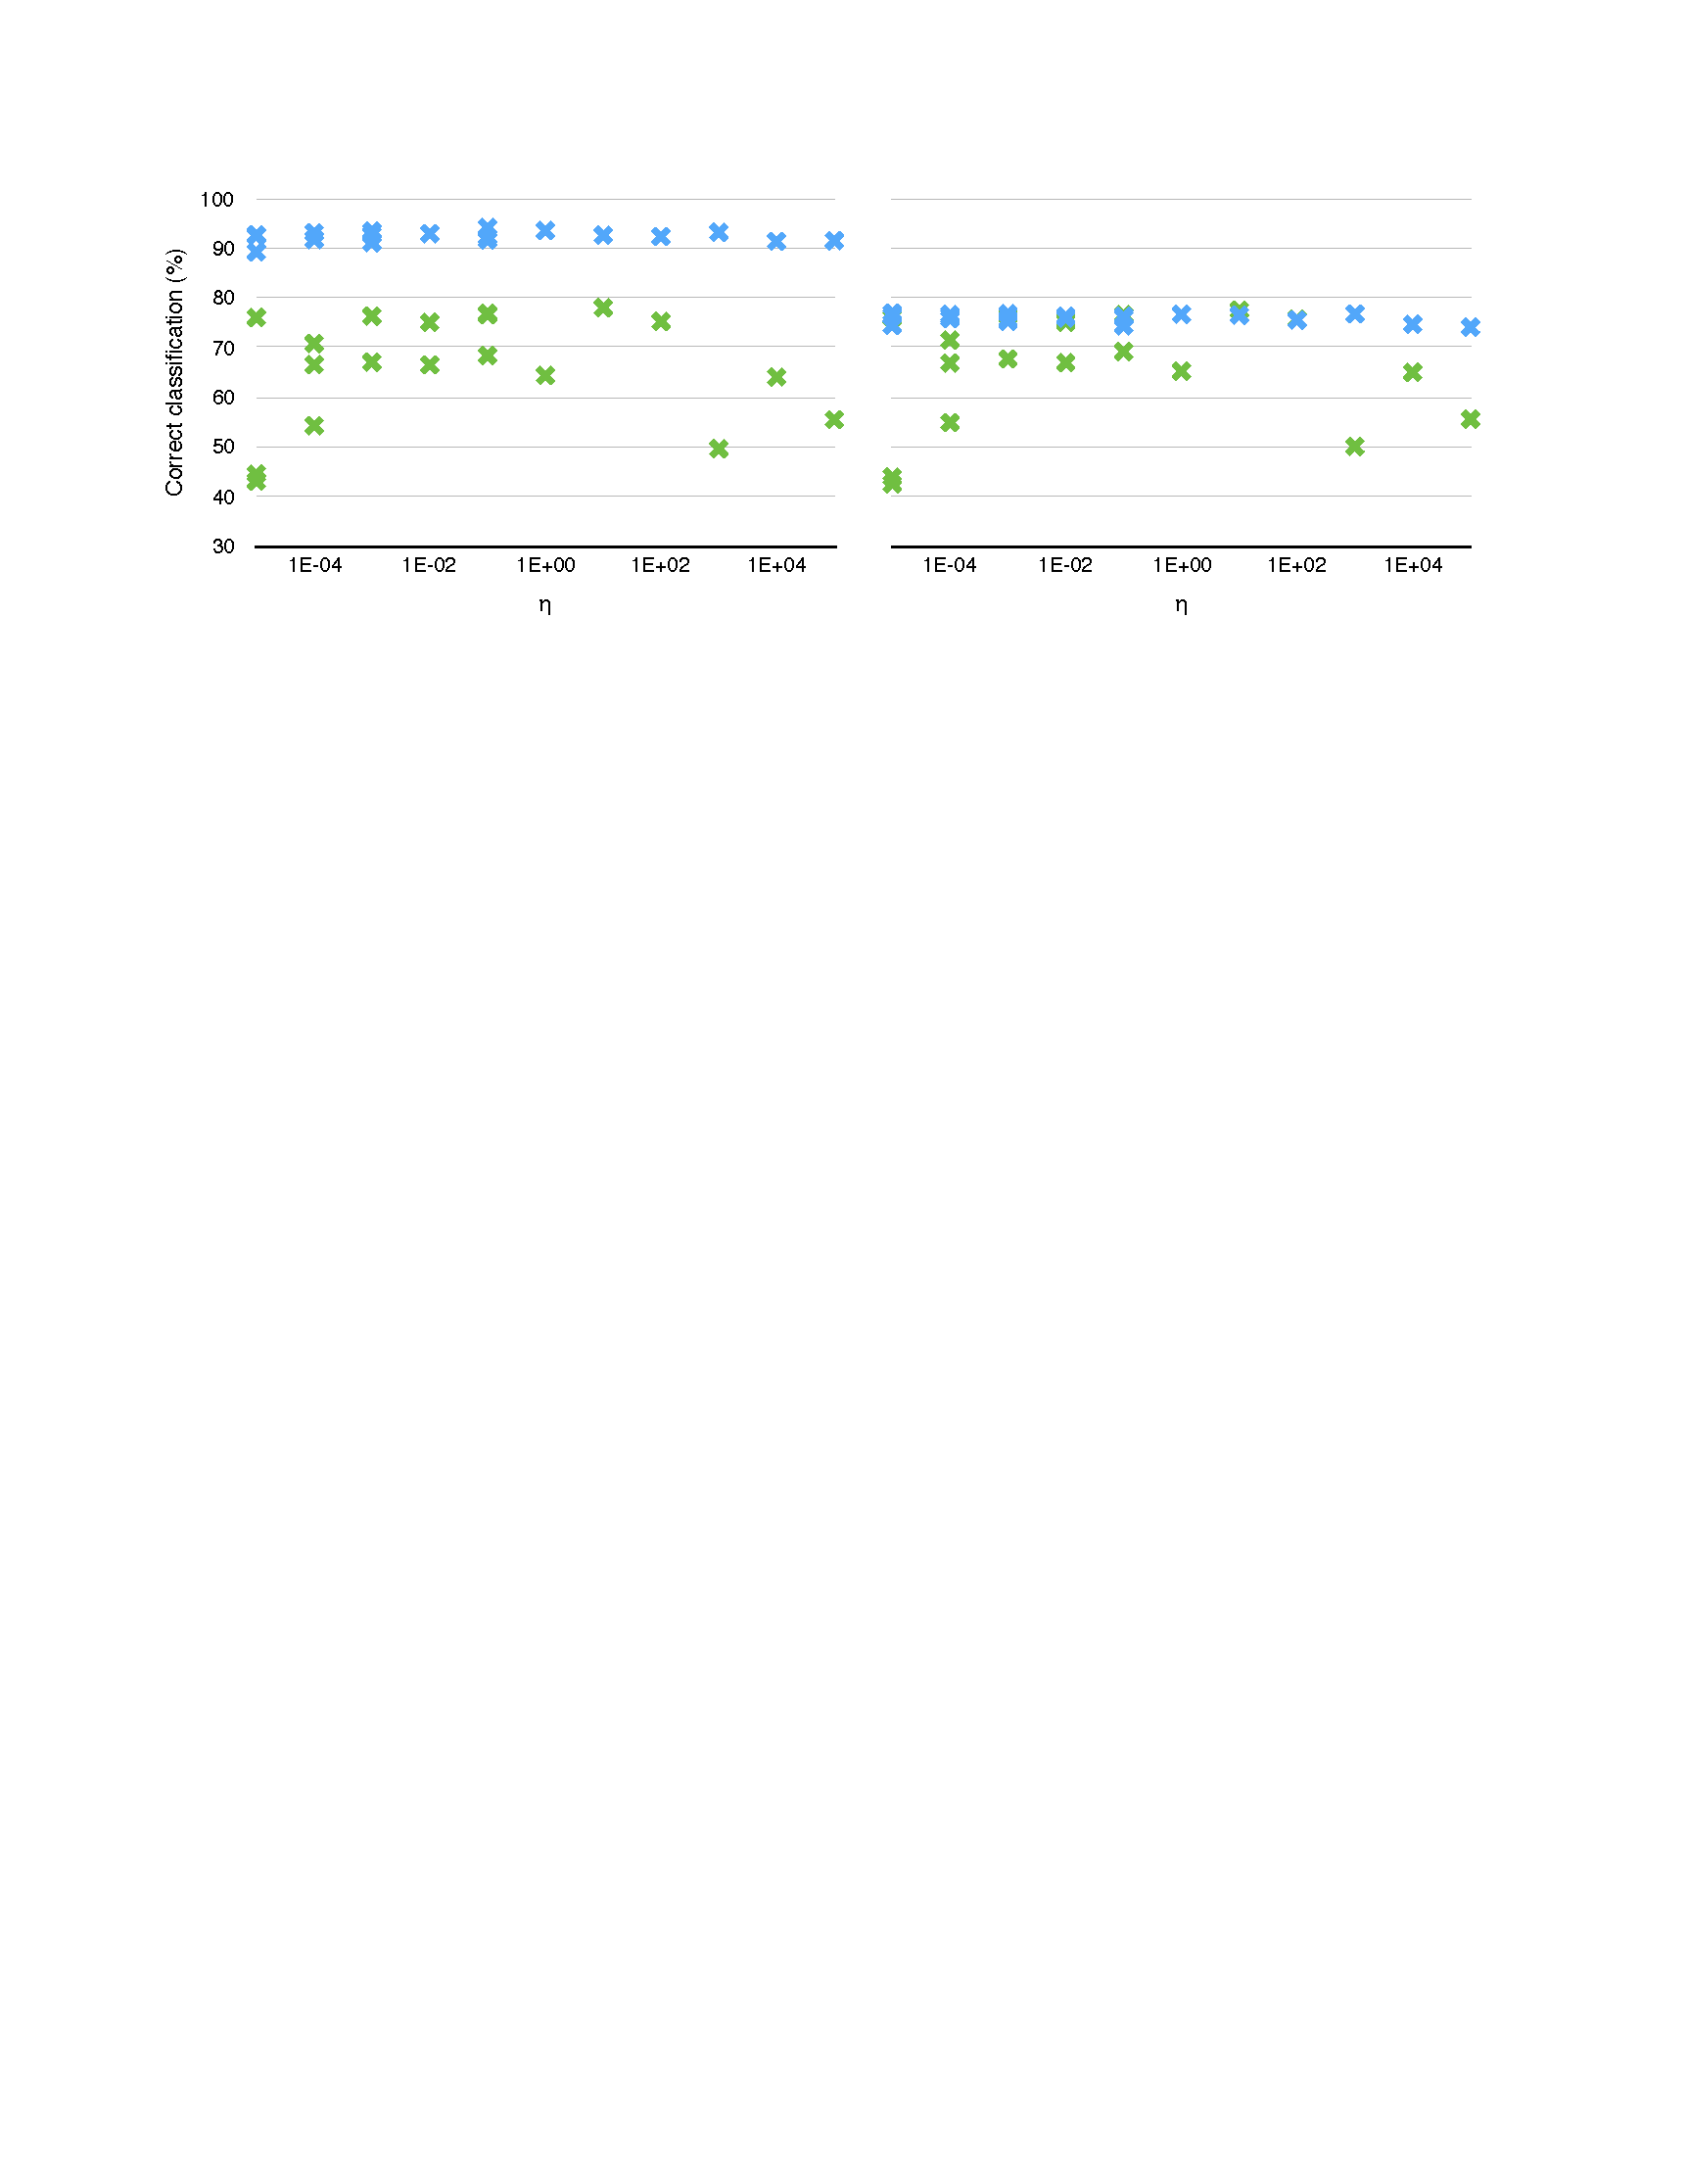
\includegraphics        [scale = 0.6]
                        {fig1.pdf}
\caption                {\small\textit{Kernelized perceptron performance\\Left: Training data; Right: Testing data\\Blue: Un-normalized; Green: Normalized}}
\label                  {fig:fig1}
\end                    {center}
\end                    {figure}

% **************************************************************************************************************************

\section                {Main Algorithms}
\label                  {sec:main_algorithms}

With the intention of developing a neural network with adversarial training in mind, a logical first step was to modify an existing neural network already in hand. Once again the SFU CMPT419/726 assignments came in useful here, with the third and final assignment involving the completion of a simple MatLab neural network for handwritten digit recognition. This code was adapted for use with the HMLC dataset, and given some further refinements such as optional training data normalization. Satisfied that the code worked as intended in this state, the adversarial components were then introduced. These additions sit entirely within the inner calculation loop, following the existing error backpropagation code lines but before the weight update step, as described in \S\ref{sec:adversarial_training}. By simply setting the perturbation size $\epsilon$ to zero, the adversarial calculations are rendered null and void, and the code performs the same as prior to their inclusion, as should be so.

Due to time restrictions, this MatLab code was unfortunately not translated into a more general language such as Python, which, as mentioned in \S\ref{sec:baseline_algorithms}, would have allowed ease of use of a greater fraction of training data. However, in the interests of time even the kernelized perceptron was run on only 10\% of the full HMLC training data, as mentioned in \S\ref{sec:kernelized_perceptron}, despite being able to handle larger datasets than its MatLab version. The MatLab neural network could comfortably be run in the same way, so with 20,000 examples for training and 5,000 examples for testing. The weight update step size for these tests was maintained at a constant $10^{-5}$, with the perturbation size $\epsilon$ scanned in the range $0\le\epsilon\le10^{-1}$. The level of adversarial training is directly proportional to $\epsilon$, so with $\epsilon=0$ essentially being the same as having no adversarial component in the code at all.

Figure \ref{fig:fig2} shows the results of this testing. Like the kernelized perceptron, the MatLab neural network displays similar values for both training and testing data when normalized, but with the former noticably greater than the latter, which was not so with the kernelized perceptron results. The values for the normalized case here are similar to those towards the upper performance range of the normalized KP, but the best normalized KP values are greater than those found here. However, there is only a relatively slight variation with $\epsilon$, to be discussed shortly, whereas the normalized KP values have much greater spread overall. So regardless of the better performance coming from the normalized KP rather than the normalized neural network, the latter code gives the impression of being more stable and consistent.

The most stark contrast between the KP and MatLab neural network is in going from normalized to un-normalized data. Normalization was deemed to be a hindrance for the KP, but it seems to be beneficial for the MatLab neural network. Not only is performace better in the normalized case for the training data, but the relative gains for the testing data seem greater still i.e. there is a greater jump from un-normalized to normalized for the testing data than the training data. Exactly why this is the case is unknown, so without going into speculation this will have to remain a point for further investigation.

Perhaps the most crucial aspect of these tests is the effect of the adversarial perturbation size $\epsilon$, this being the key to the technique under scrutiny. Note that the $x$-axes of Figure \ref{fig:fig2} are on a log-scale, and so do not naturally show the output for $\epsilon=0$. These data points are nonetheless present on the far left of each plot by means of artificially setting $\epsilon=0$ to $\epsilon=10^{-6}$. In all cases, for both training and testing data, un-normalized and normalized, the performance seems to decrease with $\epsilon$. This trend is significantly deviated from only for the last point of the un-normalized testing data, which may just be a statistical effect. The important point is that there does seem to be a clear trend here, but, again, further investigation would be required to effectively exploit it.

\begin                  {figure}
\begin                  {center}
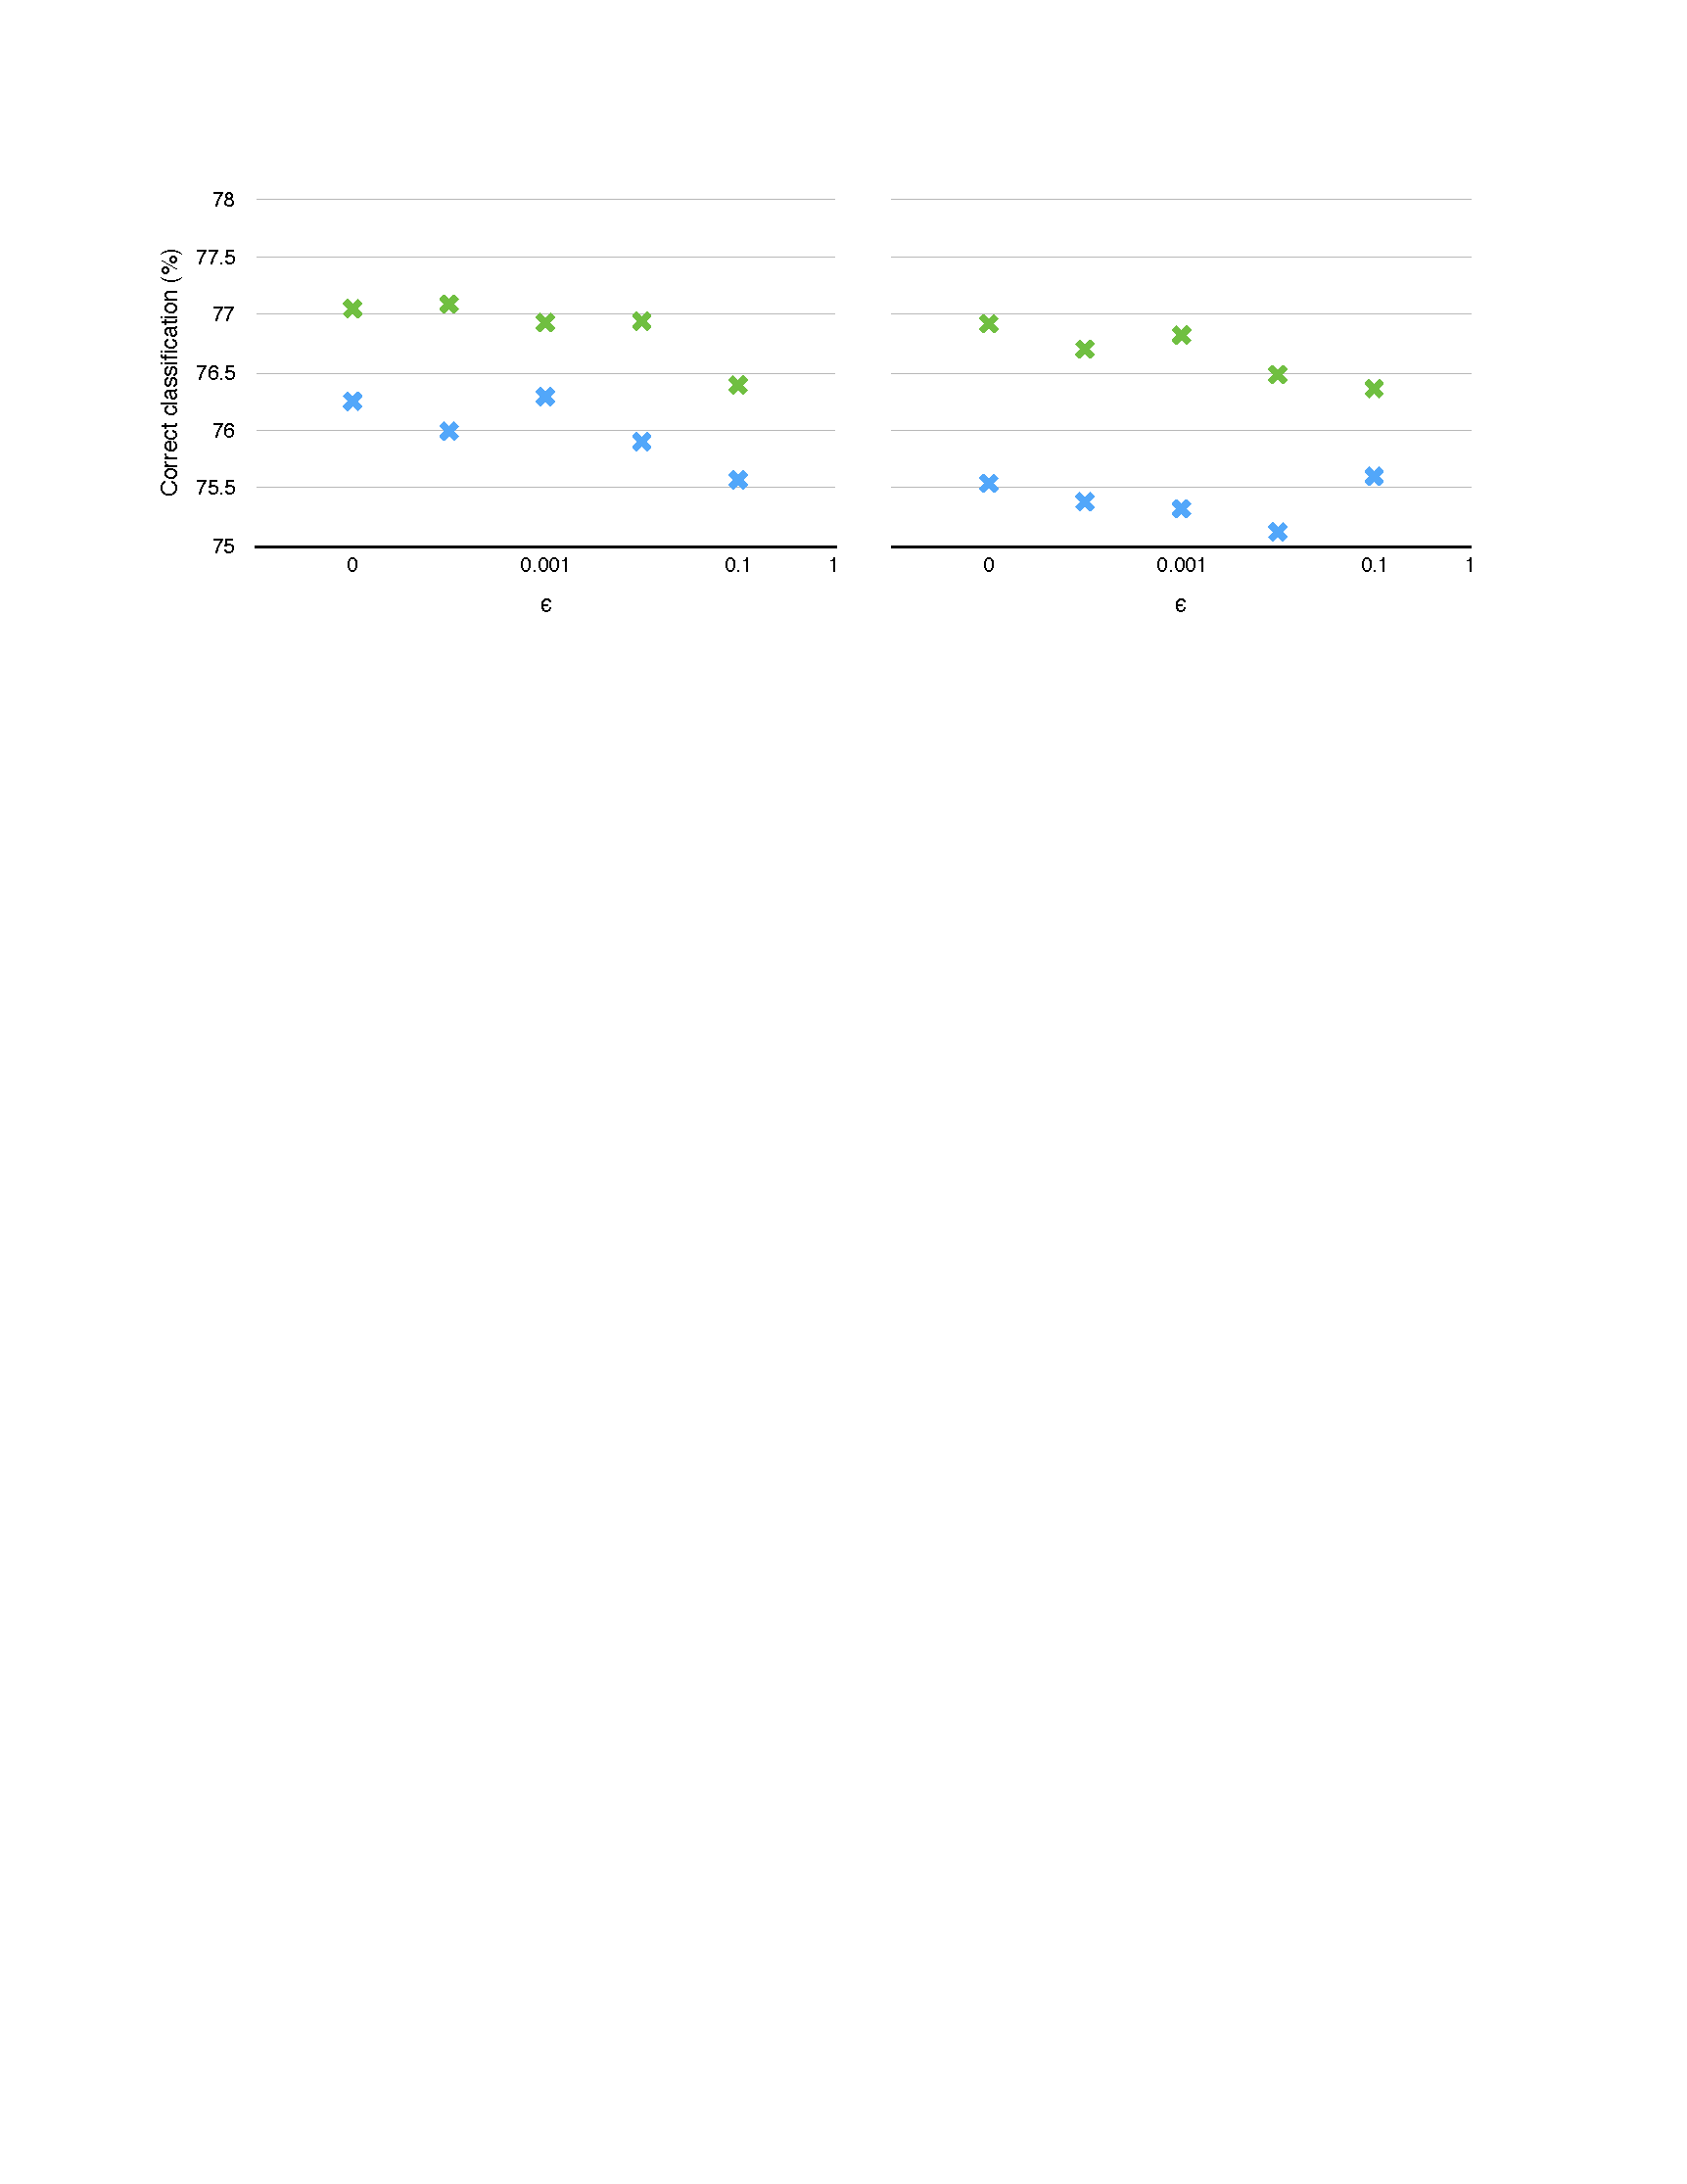
\includegraphics        [scale = 0.6]
                        {fig2.pdf}
\caption                {\small\textit{MatLab neural network performance\\Left: Training data; Right: Testing data\\Blue: Un-normalized; Green: Normalized}}
\label                  {fig:fig2}
\end                    {center}
\end                    {figure}

The MatLab neural network was intended to be no more than an advanced baseline scenario, and to provide a development platform for the adversarial training components that could then be incorporated into something more sophisticated overall. To this end, following an in-depth survey of available tools, the Python-based Theano framework was chosen as a basis for the final stage of this work. Theano is a specialized package for performing tensor computations efficiently by treating them symbollicaly. As such, it is very useful in machine learning applications. It is a competent package which is well supported and, importantly, well documented, and was a natural choice following the progression of work up to this point. Further, as the modification to the cost function $J$ required access to several gradients of the cost function, Theano's symbolic integration allowed for quick experimentation with many different cost functions. An example Theano neural network code was taken as a basis and adapted for the HMLC dataset. Specifically, a Multilayer Perceptron was written using Theano to classify the HMLC dataset. The network consisted of 30 node input layer, normalized, a hidden layer with 600 nodes and tanh as an activation function, and an output layer with two nodes, using softmax to read the output. The network was trained on a 2013 Macbook Pro with 2 cores and 8GB of ram, for 100 epochs. As with the baseline algorithms, the data was split into 225,000 training samples and 25,000 validation samples.Two cost functions were used in testing. The results are summarized below:
\begin{center}
	\begin{tabular}{|l|c|c|}
	  \hline
	  cost&non-adversarial&adversarial \\
	  \hline
	  Negative log likelihood&$73.368$&$74.552$\\
	  \hline
	  Cross entropy&$65.5$&$65.5$ \\
	  \hline
	\end{tabular}
\end{center}

% **************************************************************************************************************************

\section                {Conclusion}
\label                  {sec:conclusion}

The purpose of this project was to evaluate the affect of adding adversarial training to neural networks modeled for the Higgs Machine Learning Challenge. First, we implemented an SVM and a Kernel Perceptron. These gave us a baseline for how well simple models could perform on the challenge. Next, we added adversarial training to the neural network adapted from Assignment 3. Finally, we implemented a more robust neural network in Python using Theano. The following table shows each model implementation and its corresponding correct classification rate:

\begin{center}
	\begin{tabular}{|l|c|}
	  \hline
	  model implementation&correct validation classification percentage \\
		\hline
		SVM&$73.744$ \\
		\hline
		Kernel Perceptron&$76.98$ \\
		\hline
		Matlab NN (non-adversarial)&  \\
		\hline
		Matlab NN (adversarial)&  \\
	  \hline
	  Python/Theano NN with Negative log likelihood (non-adversarial)&$73.368$ \\
		\hline
		Python/Theano NN with Negative log likelihood (adversarial)&$74.552$ \\
	  \hline
	  Python/Theano NN with Cross entropy (non-adversarial)&$65.5$ \\
		\hline
	  Python/Theano NN with Cross entropy (non-adversarial)&$65.5$ \\
	  \hline
	\end{tabular}
\end{center}
 
The well-tuned SVM classified validation samples correctly at a rate of 73.744 percent. Similarly, the kernel perceptron classified 76.98 percent of validation samples correctly. The simple neural networks performed on par with these baseline algorithms when using a negative log likelihood cost function. Without adversarial training, the Python/Theano neural network classified 73.368 percent of validation samples correctly. This was a nearly identical success rate to the much more well-tuned SVM. Although the neural network performed slightly worse than the Kernel Perceptron, such a simple neural network shows more potential for improvement. These observations, along with the fact that the winner of the competition used neural networks, validate feet forward neural networks as a competent model for this classification problem.

Adding adversarial training to our neural networks had somewhat mixed results. In both cases where negative log likelihood was used as the cost function, adversarial training slightly improved the classification rate. On the other hand, when cross-entropy was used as the cost function, no change was observed in the classification rate between the same network with and without adversarial training on the same training and validation set. Overall, we view these results as strengthening the case for adversarial training. There were no cases where the addition of adversarial training hindered classification performance. Additionally, two of the three neural networks improved due to adversarial training.

To address the question of whether adding adversarial training is worth it or not, we examine the cost of implementation and the increased training time. In terms of implementing, the "fast gradient sign method" lives up to its name. The calculations needed to produce each adversarial sample are performed while training against the corresponding given training sample in neural networks. So, producing the adversarial samples is almost free in terms of time spent. The only significant time increase is due to training against each adversarial sample. Since every given training example produces a corresponding adversarial example, there are twice as many samples to train against when using adversarial training. Therefore, adversarial training takes twice as long as non-adversarial training in neural networks. For our simple neural networks, this increase in training time was not a problem. In general, doubling training time could be significant when cross-validating for other network parameters. However, once the other parameters have been chosen, trading a 50 percent reduction in training speed to improve a neural network classifier is generally beneficial.

The next step for our team would be to add adversarial training to the winning neural network model from the competition and test to see if it outperforms its predecessor. The improvement of our simple neural network shows promise for adversarial training to improve the winning model. Furthermore, due to the relative ease of implementation and minimal increase in training time, validating this method of adversarial training is advisable for any neural network classifier.

% **************************************************************************************************************************

               \section*{Contributions}
               \label   {sec:contributions}

\begin{itemize}
\item All: Survey of available tools; General research; Poster editing; Paper editing
\item Darren Temple: MatLab/Python kernelized perceptron adaptation; MatLab neural network adaptation; Initial adversarial training implementation; Communication with external contacts
\item Oren Shklarsky: Python SVM adaptation; Python/Theano neural network adaptation; Advanced adversarial training implementation
\item Morgan Jenkins: Interpretation of research material; Development of adversarial training algorithm; Assistance with Python/Theano neural network
\item Lola the dog: Running; Jumping; Licking heads; General distractions
\end{itemize}

% **************************************************************************************************************************

               \section*{References}
               \label   {sec:references}



% **************************************************************************************************************************


%\section{Headings: first level}
%\label{headings}
%
%First level headings are lower case (except for first word and proper nouns),
%flush left, bold and in point size 12. One line space before the first level
%heading and 1/2~line space after the first level heading.
%
%\subsection{Headings: second level}
%
%Second level headings are lower case (except for first word and proper nouns),
%flush left, bold and in point size 10. One line space before the second level
%heading and 1/2~line space after the second level heading.
%
%\subsubsection{Headings: third level}
%
%Third level headings are lower case (except for first word and proper nouns),
%flush left, bold and in point size 10. One line space before the third level
%heading and 1/2~line space after the third level heading.
%
%\section{Citations, figures, tables, references}
%\label{others}
%
%These instructions apply to everyone, regardless of the formatter being used.
%
%\subsection{Citations within the text}
%
%Citations within the text should be numbered consecutively. The corresponding
%number is to appear enclosed in square brackets, such as [1] or [2]-[5]. The
%corresponding references are to be listed in the same order at the end of the
%paper, in the \textbf{References} section. (Note: the standard
%\textsc{Bib\TeX} style \texttt{unsrt} produces this.) As to the format of the
%references themselves, any style is acceptable as long as it is used
%consistently.
%
%As submission is double blind, refer to your own published work in the 
%third person. That is, use ``In the previous work of Jones et al.\ [4]'',
%not ``In our previous work [4]''. If you cite your other papers that
%are not widely available (e.g.\ a journal paper under review), use
%anonymous author names in the citation, e.g.\ an author of the
%form ``A.\ Anonymous''. 
%
%
%\subsection{Footnotes}
%
%Indicate footnotes with a number\footnote{Sample of the first footnote} in the
%text. Place the footnotes at the bottom of the page on which they appear.
%Precede the footnote with a horizontal rule of 2~inches
%(12~picas).\footnote{Sample of the second footnote}
%
%\subsection{Figures}
%
%All artwork must be neat, clean, and legible. Lines should be dark
%enough for purposes of reproduction; art work should not be
%hand-drawn. The figure number and caption always appear after the
%figure. Place one line space before the figure caption, and one line
%space after the figure. The figure caption is lower case (except for
%first word and proper nouns); figures are numbered consecutively.
%
%Make sure the figure caption does not get separated from the figure.
%Leave sufficient space to avoid splitting the figure and figure caption.
%
%You may use color figures. 
%However, it is best for the
%figure captions and the paper body to make sense if the paper is printed
%either in black/white or in color.
%\begin{figure}[h]
%\begin{center}
%%\framebox[4.0in]{$\;$}
%\fbox{\rule[-.5cm]{0cm}{4cm} \rule[-.5cm]{4cm}{0cm}}
%\end{center}
%\caption{Sample figure caption.}
%\end{figure}
%
%\subsection{Tables}
%
%All tables must be centered, neat, clean and legible. Do not use hand-drawn
%tables. The table number and title always appear before the table. See
%Table~\ref{sample-table}.
%
%Place one line space before the table title, one line space after the table
%title, and one line space after the table. The table title must be lower case
%(except for first word and proper nouns); tables are numbered consecutively.
%
%\begin{table}[t]
%\caption{Sample table title}
%\label{sample-table}
%\begin{center}
%\begin{tabular}{ll}
%\multicolumn{1}{c}{\bf PART}  &\multicolumn{1}{c}{\bf DESCRIPTION}
%\\ \hline \\
%Dendrite         &Input terminal \\
%Axon             &Output terminal \\
%Soma             &Cell body (contains cell nucleus) \\
%\end{tabular}
%\end{center}
%\end{table}
%
%\section{Final instructions}
%Do not change any aspects of the formatting parameters in the style files.
%In particular, do not modify the width or length of the rectangle the text
%should fit into, and do not change font sizes (except perhaps in the
%\textbf{References} section; see below). Please note that pages should be
%numbered.
%
%\section{Preparing PostScript or PDF files}
%
%Please prepare PostScript or PDF files with paper size ``US Letter'', and
%not, for example, ``A4''. The -t
%letter option on dvips will produce US Letter files.
%
%Fonts were the main cause of problems in the past years. Your PDF file must
%only contain Type 1 or Embedded TrueType fonts. Here are a few instructions
%to achieve this.
%
%\begin{itemize}
%
%\item You can check which fonts a PDF files uses.  In Acrobat Reader,
%select the menu Files$>$Document Properties$>$Fonts and select Show All Fonts. You can
%also use the program \verb+pdffonts+ which comes with \verb+xpdf+ and is
%available out-of-the-box on most Linux machines.
%
%\item The IEEE has recommendations for generating PDF files whose fonts
%are also acceptable for NIPS. Please see
%\url{http://www.emfield.org/icuwb2010/downloads/IEEE-PDF-SpecV32.pdf}
%
%\item LaTeX users:
%
%\begin{itemize}
%
%\item Consider directly generating PDF files using \verb+pdflatex+
%(especially if you are a MiKTeX user). 
%PDF figures must be substituted for EPS figures, however.
%
%\item Otherwise, please generate your PostScript and PDF files with the following commands:
%\begin{verbatim} 
%dvips mypaper.dvi -t letter -Ppdf -G0 -o mypaper.ps
%ps2pdf mypaper.ps mypaper.pdf
%\end{verbatim}
%
%Check that the PDF files only contains Type 1 fonts. 
%%For the final version, please send us both the Postscript file and
%%the PDF file. 
%
%\item xfig "patterned" shapes are implemented with 
%bitmap fonts.  Use "solid" shapes instead. 
%\item The \verb+\bbold+ package almost always uses bitmap
%fonts.  You can try the equivalent AMS Fonts with command
%\begin{verbatim}
%\usepackage[psamsfonts]{amssymb}
%\end{verbatim}
% or use the following workaround for reals, natural and complex: 
%\begin{verbatim}
%\newcommand{\RR}{I\!\!R} %real numbers
%\newcommand{\Nat}{I\!\!N} %natural numbers 
%\newcommand{\CC}{I\!\!\!\!C} %complex numbers
%\end{verbatim}
%
%\item Sometimes the problematic fonts are used in figures
%included in LaTeX files. The ghostscript program \verb+eps2eps+ is the simplest
%way to clean such figures. For black and white figures, slightly better
%results can be achieved with program \verb+potrace+.
%\end{itemize}
%\item MSWord and Windows users (via PDF file):
%\begin{itemize}
%\item Install the Microsoft Save as PDF Office 2007 Add-in from
%\url{http://www.microsoft.com/downloads/details.aspx?displaylang=en\&familyid=4d951911-3e7e-4ae6-b059-a2e79ed87041}
%\item Select ``Save or Publish to PDF'' from the Office or File menu
%\end{itemize}
%\item MSWord and Mac OS X users (via PDF file):
%\begin{itemize}
%\item From the print menu, click the PDF drop-down box, and select ``Save
%as PDF...''
%\end{itemize}
%\item MSWord and Windows users (via PS file):
%\begin{itemize}
%\item To create a new printer
%on your computer, install the AdobePS printer driver and the Adobe Distiller PPD file from
%\url{http://www.adobe.com/support/downloads/detail.jsp?ftpID=204} {\it Note:} You must reboot your PC after installing the
%AdobePS driver for it to take effect.
%\item To produce the ps file, select ``Print'' from the MS app, choose
%the installed AdobePS printer, click on ``Properties'', click on ``Advanced.''
%\item Set ``TrueType Font'' to be ``Download as Softfont''
%\item Open the ``PostScript Options'' folder
%\item Select ``PostScript Output Option'' to be ``Optimize for Portability''
%\item Select ``TrueType Font Download Option'' to be ``Outline''
%\item Select ``Send PostScript Error Handler'' to be ``No''
%\item Click ``OK'' three times, print your file.
%\item Now, use Adobe Acrobat Distiller or ps2pdf to create a PDF file from
%the PS file. In Acrobat, check the option ``Embed all fonts'' if
%applicable.
%\end{itemize}
%
%\end{itemize}
%If your file contains Type 3 fonts or non embedded TrueType fonts, we will
%ask you to fix it. 
%
%\subsection{Margins in LaTeX}
% 
%Most of the margin problems come from figures positioned by hand using
%\verb+\special+ or other commands. We suggest using the command
%\verb+\includegraphics+
%from the graphicx package. Always specify the figure width as a multiple of
%the line width as in the example below using .eps graphics
%\begin{verbatim}
%   \usepackage[dvips]{graphicx} ... 
%   \includegraphics[width=0.8\linewidth]{myfile.eps} 
%\end{verbatim}
%or % Apr 2009 addition
%\begin{verbatim}
%   \usepackage[pdftex]{graphicx} ... 
%   \includegraphics[width=0.8\linewidth]{myfile.pdf} 
%\end{verbatim}
%for .pdf graphics. 
%See section 4.4 in the graphics bundle documentation (\url{http://www.ctan.org/tex-archive/macros/latex/required/graphics/grfguide.ps}) 
% 
%A number of width problems arise when LaTeX cannot properly hyphenate a
%line. Please give LaTeX hyphenation hints using the \verb+\-+ command.
%
%
%\subsubsection*{Acknowledgments}
%
%Use unnumbered third level headings for the acknowledgments. All
%acknowledgments go at the end of the paper. Do not include 
%acknowledgments in the anonymized submission, only in the 
%final paper. 
%
%\subsubsection*{References}
%
%References follow the acknowledgments. Use unnumbered third level heading for
%the references. Any choice of citation style is acceptable as long as you are
%consistent. It is permissible to reduce the font size to `small' (9-point) 
%when listing the references. {\bf Remember that this year you can use
%a ninth page as long as it contains \emph{only} cited references.}
%
%\small{
%[1] Alexander, J.A. \& Mozer, M.C. (1995) Template-based algorithms
%for connectionist rule extraction. In G. Tesauro, D. S. Touretzky
%and T.K. Leen (eds.), {\it Advances in Neural Information Processing
%Systems 7}, pp. 609-616. Cambridge, MA: MIT Press.
%
%[2] Bower, J.M. \& Beeman, D. (1995) {\it The Book of GENESIS: Exploring
%Realistic Neural Models with the GEneral NEural SImulation System.}
%New York: TELOS/Springer-Verlag.
%
%[3] Hasselmo, M.E., Schnell, E. \& Barkai, E. (1995) Dynamics of learning
%and recall at excitatory recurrent synapses and cholinergic modulation
%in rat hippocampal region CA3. {\it Journal of Neuroscience}
%{\bf 15}(7):5249-5262.
%}

\end{document}
